\documentclass[a4paper,12pt,titlepage]{article}
\usepackage[utf8]{inputenc}
\usepackage{graphicx} % Required for inserting images
\usepackage[spanish,es-tabla]{babel}
\usepackage[none]{hyphenat}
\usepackage[justification=centering]{caption}
\usepackage{subcaption}
\usepackage{amssymb,amsmath,amsthm}
\usepackage{gensymb}
\usepackage{fancyhdr}
\usepackage{wrapfig}

\lhead{Resolución de EDOs por series de potencias}
\rhead{Gonzalo Bastos González}

\pagestyle{fancy}

\title{Resolución de EDOs por series de potencias}
\author{Gonzalo Bastos González}

\newtheorem{theorem}{Teorema}
\newtheorem{mydef}{Definición}

\begin{document}

\section{Resolución de EDO de primer orden con series de potencias}

\subsection{Criterios de converxencia}

Sea a serie $\sum_{n=0}^\infty a_n$, dise que converxe se existe o seguinte límite:

\begin{equation*}
    \lim_{N \to \infty} \sum_{n=0}^N a_n
\end{equation*}

Unha condición necesaria pero non suficiente para que converxa é que:

\begin{equation*}
    \lim_{n\to \infty} a_n = 0
\end{equation*}

Para determinar a converxencia ou non converxencia dunha serie podemos utilizar diversos criterios, entre eles destacan dous, o criterio do cociente e o criterio da raíz:

\begin{itemize}
    \item O criterio do cociente se basa no cálculo deste límite:
    \begin{equation*}
        L\,=\,\operatorname*{lim}_{n\to\infty}\left|\frac{u_{n+1}}{u_{n}}\right|
    \end{equation*}
    En función do valor deste límite $L$ o criterio distingue entre tres situacións:
    \begin{enumerate}
        \item $L<1 \; \Rightarrow$ A serie converxe
        \item $L>1 \; \Rightarrow$ A serie diverxe
        \item $L=1 \; \Rightarrow$ O criterio non decide 
    \end{enumerate}
    \item O criterio da raíz se basa no cálculo do seguinte límite:
    \begin{equation*}
        \rho = \lim_{n\to\infty} \sqrt[n]{|a_n|}
    \end{equation*}
    En función do valor deste límite $\rho$ o criterio distingue entre tres situacións:
    \begin{enumerate}
        \item $\rho<1 \; \Rightarrow$ A serie converxe
        \item $\rho>1 \; \Rightarrow$ A serie diverxe
        \item $\rho=1 \; \Rightarrow$ O criterio non decide 
    \end{enumerate}
\end{itemize}

\subsection{Series de potencias}

Definimos unha serie de potencias como unha suma infinita de potencias de orden $n$, donde $x_0$ é o punto onde está centrada a serie:

\begin{equation*}
    S = \sum_{n=0}^\infty a_n(x-x_0)^n
\end{equation*}

Para $x=x_0$ a serie converxe trivialmente a $a_0$ pero para outros valores de $x$ temos que estudar a súa converxencia, aplicando o criterio do cociente en moitas ocasións:

\begin{equation*}
    L=\lim _{n \rightarrow \infty}\left|\frac{a_{n+1}\left(x-x_0\right)^{n+1}}{a_n\left(x-x_0\right)^n}\right|=\left|x-x_0\right| \lim _{n \rightarrow \infty}\left|\frac{a_{n+1}}{a_n}\right|
\end{equation*}

O valor de $L$ depende do termo $|x-x_0|$, por tanto a serie converxe $(L<1)$ se $x$ pertence ao radio de converxencia, que se define como:

\begin{equation*}
    |x-x_{0}|< \operatorname*{lim}_{n\to\infty}\left|\frac{a_{n}}{a_{n+1}}\right|\equiv R
\end{equation*}

De forma análoga se $|x-x_0|>R$ a serie diverxe. Nos extremos do intervalo $(x=x_0 \pm R)$ a serie pode ser converxente ou non, hai que estudar cada caso particular. Se no cálculo do radio de converxencia obtemos $R=0$ a serie diverxe $\forall x \in \mathbb{R}$, mentres que se $R=\infty$ entón a serie converxe $\forall x \in \mathbb{R}$. O radio de converxencia tamén se pode obter a partir do criterio da raíz:

\begin{equation*}
    R = \lim_{n\to \infty} \frac{1}{\sqrt[n]{|a_n|}}
\end{equation*}

Un exemplo de serie de potencias moi común é a que se relaciona coa exponencial:

\begin{equation*}
    e^x= \sum_{n=0}^{\infty} \frac{x^n}{n!}
\end{equation*}

Esta serie converxe $\forall x \in \mathbb{R}$, como vamos a demostrar a continuación:

\begin{equation*}
    R = \lim_{n \to \infty}\left|\frac{a_{n}}{a_{n+1}}\right| = \lim_{n \to \infty} \left |\frac{(n+1)!\,x^n}{n!\,x^{n+1}}\right | = \lim_{n \to \infty} \left |\frac{n+1}{x}\right | = \infty
\end{equation*}

\subsubsection{Propiedades das series de potencias}

Supoñamos dúas series de potencias con $R>0$ $f(x)$ e $g(x)$ centradas en $x_0$ e de término xeral $a_n$ e $b_n$ respectivamente. Algunhas das súas propiedades son:

\begin{itemize}
    \item Por definición, xa que $R>0$, $f(x)$ é \textbf{analítica} en $x_0$
    \item $f(x)+g(x)$ pode calcularse sumando termo a termo
    \item \begin{equation*}
        f(x)g(x)= \left (\sum_{n=0}^{\infty}a_n(x-x_0)^n \right )\cdot \left (\sum_{n=0}^{\infty}b_n(x-x_0)^n \right )
    \end{equation*}
    \item $f(x)$ pode integrarse termo a termo no intervalo de converxencia
    \item $f(x)$ é continua e ten derivadas continuas de todas as ordes no intervalo de converxencia que se poden calcular termo a termo:
    \begin{equation*}
        \begin{gathered}
            f'(x) = \sum_{n=1}^{\infty} na_n(x-x_0)^{n-1}\\
            f''(x) = \sum_{n=2}^{\infty} n(n-1)a_n(x-x_0)^{n-2} \\
            f'''(x)= \sum_{n=3}^{\infty} n(n-1)(n-2)a_n(x-x_0)^{n-3}
        \end{gathered}
    \end{equation*}
    A expresión da derivada n-ésima resulta ser:

    \begin{equation*}
        f^{(n)}(x_0) = n!a_n \Rightarrow a_n =\frac{f^{(n)}(x_0)}{n!}
    \end{equation*}

    Polo que a serie de potencias é a serie de Taylor no punto $x_0$:

    \begin{equation*}
        f(x)=\sum_{n=0}^{\infty} \frac{f^{(n)}(x_0)}{n!} (x-x_0)^n
    \end{equation*}
\end{itemize}

A última propiedade marca unha clara relación entre as funcións coñecidas e as súas series de Taylor. O teorema de Taylor nos di que sexa unha función $h(x)$continua e infinitamente derivable en $|x-x_0|$ podemos expresala como:

\begin{equation*}
    h(x) = \sum_{n=0}^{\infty} \frac{h^{(n)}(x_0)}{n!} (x-x_0)^n + R_N(x)
\end{equation*}

Onde o resto é $R_N(x)$, que se define como:

\begin{equation*}
    R_N(x) \frac{h^{N+1}(\overline{x})}{(N+1)!}(x-x_0)^{N+1}
\end{equation*}

Non obstante o teorema de Taylor non asegura que a serie de potencias sea converxente $\forall x \in \mathbb{R}$, a función só se pode expesar como serie de potencias nun determinado intervalo, no que se cumpre que:

\begin{equation*}
    \lim_{N\to \infty}R_N(x)=0
\end{equation*}

\subsection{A ecuación $y'=y$}

A solución de esta ED é ben coñecida, $y=Ce^x$, pero vamos a obtela a partir de series de potencias:

\begin{equation*}
    \begin{gathered}
        y = \sum_{n=0}^{\infty} a_nx^n \\
        y' = \sum_{n=1}^{\infty} na_n(x-x_0)^{n-1} \overbrace{=}^{\text{Buscamos $x^n$}} = \sum_{n=0}^{\infty} a_{n+1}(n+1)x^{n}
    \end{gathered}
\end{equation*}

Sustituimos na ED e igualamos os coeficientes:

\begin{equation*}
    a_n= a_{n+1}(n+1) \Rightarrow a_{n+1}=\frac{a_n}{n+1}
\end{equation*}

Unha vez obtida a relación de recorrencia vamos a buscar o termo xeral $a_n$:

\begin{equation*}
    \begin{array}{ll}
    n=0 \Rightarrow \quad a_1=\frac{a_0}{1}=a_0 ; & n=1 \Rightarrow a_2=\frac{a_1}{2}=\frac{a_0}{2} \\
    n=2 \Rightarrow \quad a_3=\frac{a_2}{3}=\frac{a_0}{3 \cdot 2} ; & n=3 \Rightarrow a_4=\frac{a_3}{4}=\frac{a_0}{4 \cdot 3 \cdot 2} \quad \cdots
    \end{array}
\end{equation*}

Por tanto, o termo xeral da serie é:

\begin{equation*}
    a_n=\frac{a_0}{n!}
\end{equation*}

Por tanto a expresión final da serie de potencias sería:

\begin{equation*}
    y = \sum_{n=0}^{\infty} \frac{a_0}{n!}x^n = a_0 \sum_{n=0}^{\infty} \frac{x^n}{n!}
\end{equation*}

Unha vez coñecida a serie debemos estudar a súa converxencia, neste caso é moi sinxelo pois é a serie da exponencial, que como demostramos anteriormente converxe $\forall x \in \mathbb{R}$. A solución final é $y = a_0e^x$.

\subsection{A serie do binomio}

Este método de resolución é moi útil para coñecer a serie de Taylor dunha determinada función coñecida unha ecuación diferencial que a función satisfaga. En concreto vamos a estudar a función do binomio:

\begin{equation*}
    y = (1+x)^p \quad \text{con} \; p\in\mathbb{R}
\end{equation*}

Esta función cumple a seguinte ecuación diferencial:

\begin{equation*}
    (1+x)y'=py \quad \text{con} \; y(0)=1
\end{equation*}

Vamos a buscar unha solución por series de potencias arredor de $x_0=0$, o que nos permite calcular $y$ e $y'$ como:

\begin{equation*}
    \begin{gathered}
        y = \sum_{n=0}^{\infty} a_nx^n \\
        y' = \sum_{n=1}^{\infty} na_n(x-x_0)^{n-1}
    \end{gathered}
\end{equation*}

Para sustituir na ED primeiro vamos a operar o paréntesis para facilitar as operacións:

\begin{equation*}
    \begin{gathered}
        \text{ED:} \quad y' +xy'=py \\
        xy' = \sum_{n=1}^{\infty} na_nx^n
    \end{gathered}
\end{equation*}

Sustituindo todas as expresións na ED obtemos que:

\begin{equation*}
    \begin{gathered}
        \sum_{n=1}^{\infty} na_n(x-x_0)^{n-1} + \sum_{n=1}^{\infty} na_nx^n = p\sum_{n=0}^{\infty}a_nx^n\\
        \sum_{n=0}^{\infty} (n+1)a_{n+1}(x-x_0)^{n} + \sum_{n=0}^{\infty} na_nx^n = p\sum_{n=0}^{\infty}a_nx^n\\
        \sum_{n=0}^{\infty} [na_n+(n+1)a_{n+1}]x^n= p\sum_{n=0}^{\infty}a_nx^n \\
        na_n+(n+1)a_{n+1} = pa_n \quad n=0,1,2,... \\
        a_{n+1} = \frac{p-n}{n+1}a_n
    \end{gathered}
\end{equation*}

\newpage

Unha vez obtida a relación de recorrencia vamos a buscar o termo xeral $a_n$ por inducción dando valores a $n$:

\begin{equation*}
    \begin{array}{l}
        n=0  \Rightarrow a_1 = pa_0 \\
        n=1 \Rightarrow a_2 = \frac{p-1}{2} a_0 = \frac{p(p-1)}{2}a_0 \\
        n=2 \Rightarrow a_3 = \frac{p-2}{3}a_2 = \frac{p(p-1)(p-2)}{3\cdot2}a_0 \\
        n = 3 \Rightarrow \frac{p-3}{4}a_3 = \frac{p(p-1)(p-2)(p-3)}{4\cdot 3\cdot2}a_0
    \end{array}
\end{equation*}

Por inducción podemos ver que o termo xeral é:

\begin{equation*}
    a_n = \frac{p(p-1)(p-2)\cdots (p-n+1)}{n!}a_0
\end{equation*}

Como a ED ten a condición de $y(0)=1$ a denominada serie do binomio queda da seguinte forma:

\begin{equation*}
    (1+x)^p= 1 + \sum_{n=1}^{\infty} \frac{p(p-1)(p-2)\cdots (p-n+1)}{n!} x^n
\end{equation*}

Esta serie queda en función do parámetro $p$, dependendo do seu valor a serie vai ter comportamentos diferentes. O caso máis común é o de $p\in \mathbb{N}$. Neste caso os coeficientes a partir de $a_{p+1}$ se cancelan (Teñen o termo $p-(p-1)+1=0$ multiplicando no numerador) polo que a suma se reduce a unha suma finita, trúncase. Ademais mentres que $p\geq n$ cúmplese que:

\begin{equation*}
    p(p-1)(p-2)\cdots (p-n+1) = \frac{p!}{(p-n)!}
\end{equation*}

Polo que podemos escribir a serie como o binomio de Newton:

\begin{equation*}
    (1+x)^p = \sum_{n=0}^p \frac{p!}{n!(p-n)!}x^n = \sum_{n=0}^p \binom{p}{n} \quad p\in \mathbb{N}
\end{equation*}

No caso de $p\notin \mathbb{N}$ podemos estudar a converxencia da serie co criterio do cociente (Empregando a relación de recorrencia):

\begin{equation*}
    R=\lim_{n\to \infty}\left |\frac{a_n}{a_{n+1}}\right | = \lim_{n\to \infty} \left |\frac{n+1}{p-n}\right | = 1
\end{equation*}

Polo tanto, se $p\notin \mathbb{N}$ a serie converxe se $|x|<1$ e diverxe se $|x|>1$.

\newpage

\section{A función Gamma de Euler}

Esta función nos permite unha xeralización da función factorial ($p!$) cando $p\notin \mathbb{N}$. Defínese como:

\begin{equation*}
    \Gamma(p) = \int_{0}^{\infty} t^{p-1}e^{-t}dt \quad 0<p\in \mathbb{R}
\end{equation*}

A propiedade principal desta función é a que relaciona dous términos consecutivos:

\begin{equation*}
    \Gamma(p+1) = p\Gamma(p)
\end{equation*}

Podemos demostrala integrando por partes:

\begin{equation*}
    \begin{gathered}
        \Gamma(p+1) = \int_0^{\infty} t^pe^{-t}dt \overset{\begin{array}{l}
            u=t^p \rightarrow du=pt^{p-1}\\
            dv=e^{-t} \rightarrow v = -e^{-t} \end{array}}{=} \\ =-t^pe^{-t}\Big|_0^{\infty} + p\int_{0}^{\infty} t^{p-1}e^{-t}dt = p\Gamma(p)
    \end{gathered}
\end{equation*}

Vamos a calcular $\Gamma(1)$ e logo para o resto de valores tales que $p\in \mathbb{N}$ por recurrencia:

\begin{equation*}
    \begin{array}{l}
        \Gamma(1) = \int_0^{\infty} e^{-t}dt = -e^{-t}\Big|_0^{\infty} = 1 = 0! \\
        \Gamma(2) =1\Gamma(1)=1\cdot1=1!\\
        \Gamma(3) =2 \Gamma(2) = 2\cdot 1 \cdot 1 = 2!\\
        \Gamma(4) = 3\Gamma(3) = 3 \cdot 2\cdot 1 \cdot 1 = 3! \\
        \Gamma(5) = 4\Gamma(4) = 4 \cdot3 \cdot 2\cdot 1 \cdot 1 = 5!
    \end{array}
\end{equation*}

Por inducción demostramos a relación que hai entre o factorial e a función gamma:

\begin{equation*}
    \Gamma(n+1)=n! \quad n\in\mathbb{N}
\end{equation*}

Unha vez coñecidos os valores da función gamma nos naturais temos que estendela a toda a recta real. Un caso particular que ten un resultado analítico simple é $\Gamma(\frac{1}{2})$:

\begin{equation*}
    \Gamma\left (\frac{1}{2}\right ) = \int_0^{\infty} \frac{e^{-t}}{\sqrt{t}}dt \overset{t = s^2}{=} 2\int_0^{\infty} e^{-s^2} ds
\end{equation*}

\newpage

Obtemos así a integral da metade da gaussiana, que por ser unha función par podemos cambiar o límite de integración:

\begin{equation*}
    2\int_0^{\infty} e^{-s^2} ds = \int_{-\infty}^{\infty} e^{-s^2} ds = \sqrt{\pi}
\end{equation*}

Desta forma obtivemos o seguinte resultado, que nos permite calcular factoriales de números non enteiros negativos:

\begin{equation*}
    \Gamma \left (\frac{1}{2}\right ) = \sqrt{\pi} = \left (-\frac{1}{2}\right )!
\end{equation*}

Aplicando a relación de recorrencia $\Gamma(p+1) = p\Gamma(p)$ podemos calcular o valor da función gamma para calquera semienteiro positivo, por exemplo:

\begin{equation*}
    \Gamma\left (\frac{3}{2}\right ) = \Gamma \left (\frac{1}{2} + 1\right ) = \frac{1}{2} \Gamma\left (\frac{1}{2}\right ) = \frac{\sqrt{\pi}}{2} = \left (\frac{1}{2}\right )!
\end{equation*}

\begin{figure}[h!]
    \centering
    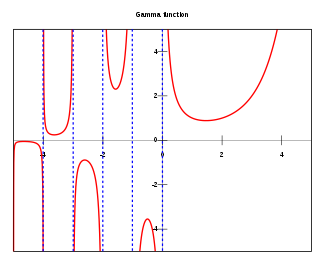
\includegraphics[width=0.85\linewidth]{Images/gammagrafica.png}
    \caption{Gráfica de $\Gamma(p)$}
\end{figure}

Se reescribimos a relación de recorrencia como:

\begin{equation*}
    \Gamma(p) = \frac{\Gamma(p+1)}{p}
\end{equation*}

Podemos extender aos semienteiros negativos o procedemento anterior para obter resultados analíticos, un exemplo sería:

\begin{equation*}
    \Gamma(-\frac{1}{2}) = \frac{\Gamma(-\frac{1}{2}+1)}{-\frac{1}{2}} = -2\sqrt{\pi}
\end{equation*}

Podemos aplicar esta misma lóxica para calcular o valor da función no intervalo $(-1,0)$ a partir dos seus valores no intervalo $(0,1)$ e así sucesivamente. Esta extensión é válida $\forall x <0 | x\notin \mathbb{Z}$. Nos valores enteiros a función non está definida porque tampouco o está no cero:

\begin{equation*}
    \lim_{p\to0} \Gamma(p) = \lim_{p\to 0} \frac{\Gamma(p+1)}{p} =\lim_{p\to0} \frac{1}{p} = \pm \infty
\end{equation*}

En consecuencia a función tampouco está definida en ningún dos enteiros negativos, probarémolo para $p=-1$:

\begin{equation*}
    \lim_{p\to-1} = \lim_{p\to-1} \frac{\Gamma(p+1)}{p} = \lim_{p\to-1} \frac{\Gamma(0)}{-1} = \pm \infty
\end{equation*}

Por último, podemos relacionar os valores da función gamma de dous números que disten entre si un enteiro:


\begin{align*}
    \Gamma(p+1)&=p\Gamma(p)\\ &= p(p-1)\Gamma(p-1)\\ &= p(p-1)(p-2)\Gamma(p-2) \\ &= p(p-1)(p-2) \cdots (p+1-n)\Gamma(p+1-n)
\end{align*}

O producto anterior aparece tamén na serie do binomio, polo que podemos reescribila como:

\begin{equation*}
    (1+x)^p = \sum_{n=0}^{\infty} \frac{\Gamma(p+1)}{n!\Gamma(p+1-n)} \quad \left\{ \begin{array}{lc}
        \text{Se} \; p=0,1,2,... & \forall x \\
        \text{Se} \; p \neq 0,1,2,... & |x|<1
    \end{array} \right.
\end{equation*}

\newpage

\section{Resolución de EDO de segunda orde}

\subsection{Puntos singulares e ordinarios}

Vamos a considerar a seguinte ED en forma normal (Se non o está hai que normalizala!!):

\begin{equation*}
    y'' +P(x)y' + Q(x)y =0
\end{equation*}

\begin{mydef}
Por definición diremos que $x_0$ é un punto ordinario se $P(x)$ e $Q(x)$ son analíticas nese punto. Se o punto non é ordinario denomínase singular.
\end{mydef}

\begin{theorem}
    Sexa $x_0$ un punto ordinario e sexan $a_0$ e $a_1$ constantes arbitrarias. Existe unha función $f(x)$ analítica en $x_0$ que verifica a ED e as condicións iniciais de $y(x_0)=a_0$ e $y'(x_0)=a_1$.
    \par Ademais cúmplese que o radio de converxencia do desenvolvemento en series da solución é, polo menos, o menor dos radios dos desenvolvementos en serie de Taylor de $P(x)$ e $Q(x)$.
\end{theorem}

\subsection{Ecuacións de Legendre}

Denominamos funcións de Legendre á familia de funcións que verifican a seguinte ED:

\begin{equation*}
    (1-x^2)y''-2xy'+p(p+1)y=0 \quad p \in \mathbb{R}
\end{equation*}

En forma normal:

\begin{equation*}
    y'' - \frac{2x}{1-x^2}y'+ \frac{p(p+1)}{1-x^2}y=0
\end{equation*}

Polo tanto as funcións $P(x)$ e $Q(x)$ son:

\begin{equation*}
    \left.
    \begin{array}{c}
        P(x)= - \frac{2x}{1-x^2} \\
        Q(x) = \frac{p(p+1)}{1-x^2}  
    \end{array}
    \right\}\Rightarrow \text{Analíticas en $x_0=0$ con $R=1$} 
\end{equation*}

Vamos a buscar unha solución xeral da forma $y=\sum_{n=0}^{\infty} a_nx^n$, calculando o resto de termos implicados na ecuación:

\begin{equation*}
    \begin{gathered}
        y' = \sum_{n=0}^{\infty} na_nx^{n-1} \Rightarrow -2xy' = -\sum_{n=0}^{\infty} 2na_nx^n\\
        y'' = \sum_{n=2}^{\infty} n(n-1)a_nx^{n-2} \Rightarrow \sum_{n=0}^{\infty} (n+2)(n+1)a_nx^{n} \\
        -x^2y'' = - \sum _{n=2}^{\infty} n(n-1)a_n x^n \Rightarrow - \sum _{n=0}^{\infty} n(n-1)a_n x^n
    \end{gathered}
\end{equation*}
No paso intermedio da segunda liña definimos un cambio de variable $j = n-2$ e despois cambiando $j$ por $n$. Podemos facer isto porque o índice é unha variable muda, que solo existe dentro do sumatorio. Unha vez temos os nosos sumatorios cos índices iguais podemos sustituir na ED:

\begin{equation*}
    \begin{gathered}
    \sum_{n=2}^{\infty} n(n-1)a_nx^{n-2} - \sum _{n=0}^{\infty} n(n-1)a_n x^n -\sum_{n=0}^{\infty} 2na_nx^n + \sum_{n=0}^{\infty}p(p+1)a_nx^n = 0 \Rightarrow \\
    \sum_{n=0}^{\infty} [(n+2)(n+1)a_{n+2}-[n(n-1)-2n+p(p+1)]a_n]x^n = 0
    \end{gathered}
\end{equation*}

Temos unha serie de Taylor igualada a función 0, polo que podemos igualar todos os termos a 0:

\begin{equation*}
    \begin{gathered}
        (n+2)(n+1)a_{n+2}-[n(n-1)-2n+p(p+1)]a_n = 0 \quad n=0,1,2,... \\
        (n+2)(n+1)a_{n+2} - (p-n)(p+n-1)a_n = 0
    \end{gathered}
\end{equation*}

Así calculamos a relación de recorrencia:

\begin{equation*}
    a_{n+2} = -\frac{(p-n)(p+n+1)}{(n+1)(n+2)} a_{n} \quad n=0,1,2,...
\end{equation*}

\begin{equation*}
\begin{aligned}
    & a_{2}=-\frac{p(p+1)}{1 \cdot 2} a_{0} \\
    & a_{4}=-\frac{(p-2)(p+2+1)}{3 \cdot 4} a_{2} \quad=\quad \frac{(p-2) p(p+1)(p+3)}{4 !} a_{0} \\
    & a_{6}=-\frac{(p-4)(p+4+1)}{5 \cdot 6} a_{4} \quad=-\frac{(p-4)(p-2) p(p+1)(p+3)(p+5)}{6 !} a_{0}
\end{aligned}
\end{equation*}

Estes termos se relacionan mediante índices pares, os termos de índices impares siguen unha recorrencia indepente, non hai conexión entre os termos pares e os impares. Os termos impares $a_{2n+1}$ seguen a seguinte relación:

\begin{equation*}
\begin{aligned}
    & a_{3}=-\frac{(p-1)(p+2)}{2 \cdot 3} a_{1} \\
    & a_{5}=-\frac{(p-3)(p+3+1)}{4 \cdot 5} a_{3}=\frac{(p-3)(p-1)(p+2)(p+4)}{5 !} a_{1} \\
    & a_{7}=-\frac{(p-5)(p+5+1)}{6 \cdot 7} a_{5}=-\frac{(p-5)(p-3)(p-1)(p+2)(p+4)(p+6)}{7 !} a_{1}
\end{aligned}
\end{equation*}

Polo tanto, temos dúas solucións LI que depende de $a_0$ e de $a_1$, como nos expresaba o Th.1. Este resultado ten moito sentido, pois as constantes $a_0$ e $a_1$ son as constantes da ED, que ten 2 por ser de segundo grao.

\begin{equation*}
\begin{aligned}
& y_{1}=1-\frac{p(p+1)}{2 !} x^{2}+\frac{(p-2) p(p+1)(p+3)}{4 !} x^{4} \\
& -\frac{(p-4)(p-2) p(p+1)(p+3)(p+5)}{6 !} x^{6}+\cdots \\
& y_{2}=x-\frac{(p-1)(p+2)}{3 !} x^{3}+\frac{(p-3)(p-1)(p+2)(p+4)}{5 !} x^{5} \\
& -\frac{(p-5)(p-3)(p-1)(p+2)(p+4)(p+6)}{7 !} x^{7}+\cdots
\end{aligned}
\end{equation*}

Estas dúas solucións denomínanse \textbf{funcións de Legendre}. Estas funcións son unha serie infinita de potencias, cuxa converxencia estudaremos a continuación.

\subsection{Converxencia e polinomios de Legendre}

Se $p\in \mathbb{Z}$ a serie trúncase nun momento dado, coverténdose nun polinomio finito. Se $p$ é par e positivo ou impar e negativo trúncase $y_1$, mentres que se $p$ é impar e positivo ou par e negativo, trúncase $y_2$. No caso de que $p\notin \mathbb{Z}$ vamos a estudar a converxencia aplicando o criterio do cociente, por exemplo a $y_1$:

$$
L=\lim _{n \rightarrow \infty}\left|\frac{a_{2 n+2} x^{2 n+2}}{a_{2 n} x^{2 n}}\right|=x^{2} \lim _{n \rightarrow \infty}\left|\frac{(p-2 n)(p+2 n+1)}{(2 n+1)(2 n+2)}\right|=x^{2}
$$

Polo tanto, a serie converxe se $|x|<1$. A demostración para $y_2$ é análoga.

\par O caso máis interesante é aquel no que $p=L\in \mathbb{Z}$. Neste caso consideraremos só as series que quedan truncadas. Ademais, en vez de usar as funcións $y_1$ e $y_2$, soen multiplicarse por unha constante de xeito que o coeficiente que acompaña a potencia máis alta sexa:

\begin{equation*}
    a_L = \frac{(2 L) !}{2^{L}(L !)^{2}}=\frac{(2 L-1)(2 L-3)(2 L-5) \cdots \quad 7 \cdot 5 \cdot 3 \cdot 1}{L !}
\end{equation*}

Polo tanto as novas funcións, os \textbf{polinomios de Legendre}, quedan da seguinte forma:

\begin{equation*}
    P_{L}(x)=\sum_{k=0}^{[L / 2]} \frac{(-1)^{k}(2 L-2 k) !}{2^{L} k !(L-k) !(L-2 k) !} x^{L-2 k}
\end{equation*}

onde $[L / 2]$ é o maior enteiro menor ou igual a $L / 2$ :

$$
[L / 2]= \begin{cases}L / 2 & \text { se } L \text { par } \\ (L-1) / 2 & \text { se } L \text { impar }\end{cases}
$$  

A forma máis útil de facer os cálculos dos polinomios de Legendre é empregando a fórmula de Rodrigues:

\begin{equation*}
    P_{L}(x)=\frac{1}{2^{L} L !} \frac{\mathrm{d}^{L}}{\mathrm{~d} x^{L}}\left[\left(x^{2}-1\right)^{L}\right], \quad L \in \mathbb{N}_{0}
\end{equation*}

Para $L=0$ obtemos a recta $y=1$, para $L=1$ obtemos a recta $y=x$, para $L=2$ obtemos o seguinte polinomio:

\begin{equation*}
    P_2(x) = \frac{1}{2^22!} \frac{d^2}{dx^2}[(x^2-1)^2] = \frac{1}{8} \frac{d^2}{dx^2}[x^4-2x^2+1] = \frac{3x^2-1}{2}
\end{equation*}


\par Na seguinte figura podemos ver representados polinomios de Legendre ata orde 5, con $p=n$:

\begin{figure}[h!]
    \centering
    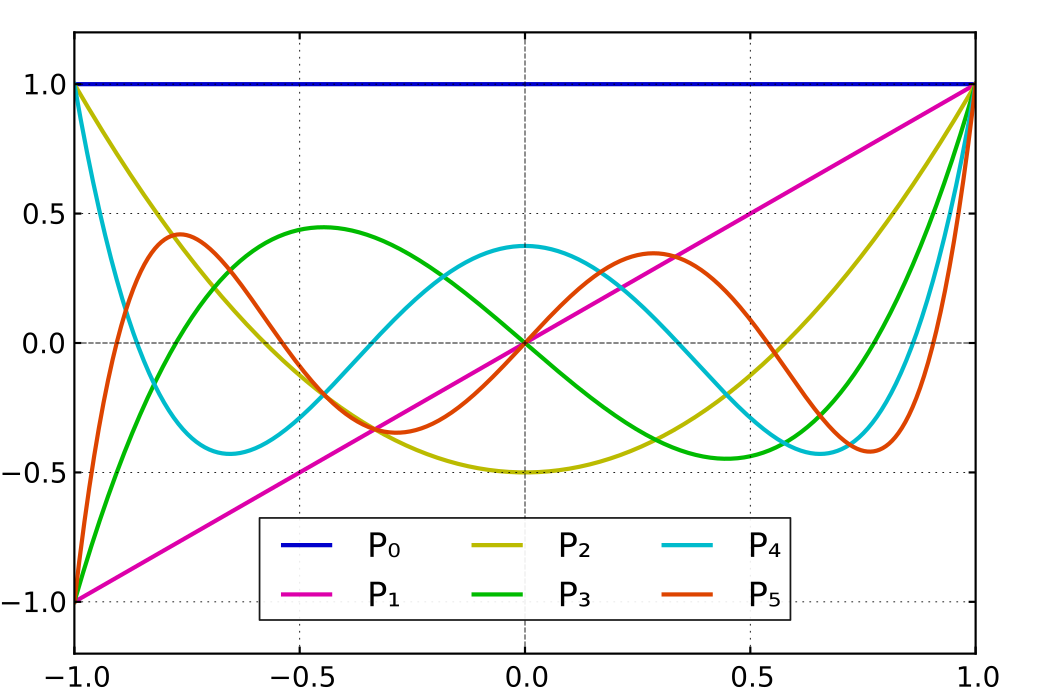
\includegraphics[width=0.8\linewidth]{Images/legendre.png}
    \caption{Polinomios de Legendre}
\end{figure}

Onde os polinomios teñen as seguintes ecuacións:

\begin{equation*}
    \begin{gathered}
        P_3(x)= \frac{5x^3-3x}{2} \\
        P_4(x) = \frac{35x^4-30x^2+3}{8}\\
        P_5(x) = \frac{63x^5-70x^3+15x}{8}
    \end{gathered}
\end{equation*}

\subsection{Algunhas propiedades}
Os polinomios de Legendre:

\begin{itemize}
  \item verifican $P_{L}(1)=1$ e $P_{L}(-1)=(-1)^{L}$
  \item son ortogonais: $\int_{-1}^{1} P_{L}(x) P_{L^{\prime}}(x) \mathrm{d} x=0$ se $L \neq L^{\prime}$
\end{itemize}

\section{Puntos singulares e series de Frobenius}

\subsection{Introdución}
Partimos dunha ecuación de Euler de segunda orde da forma:

\begin{equation*}
    x^2 y^{\prime \prime}+p x y^{\prime}+q y=0
\end{equation*}

Onde $p,q \in \mathbb{R}$ son constantes. Escribindo en forma normal a ecuación temos que:

\begin{equation*}
    y^{\prime \prime}+\frac{p}{x} y^{\prime}+\frac{q}{x^{2}} y=0
\end{equation*}

En $x_0=0$ a función ten un punto non ordinario xa que as funcións $P(x)$ e $Q(x)$ non son analíticas. Non podemos aplicar o Th.1 para afirmar que existen solucións, pero por ser unha ecuación de Euler sabemos que existen solucións da forma:

\begin{equation*}
    y = x^m
\end{equation*}

Respecto a estas solucións temos que notar que, salvo que $m\in\mathbb{N}$, non son infinitamente derivables en $x_0=0$, por iso non son analíticas.

\begin{equation*}
    y^{k)}=m(m-1) \cdots(m-k+1) x^{m-k}
\end{equation*}

\begin{wrapfigure}{r}{0.5\textwidth}
    \centering
    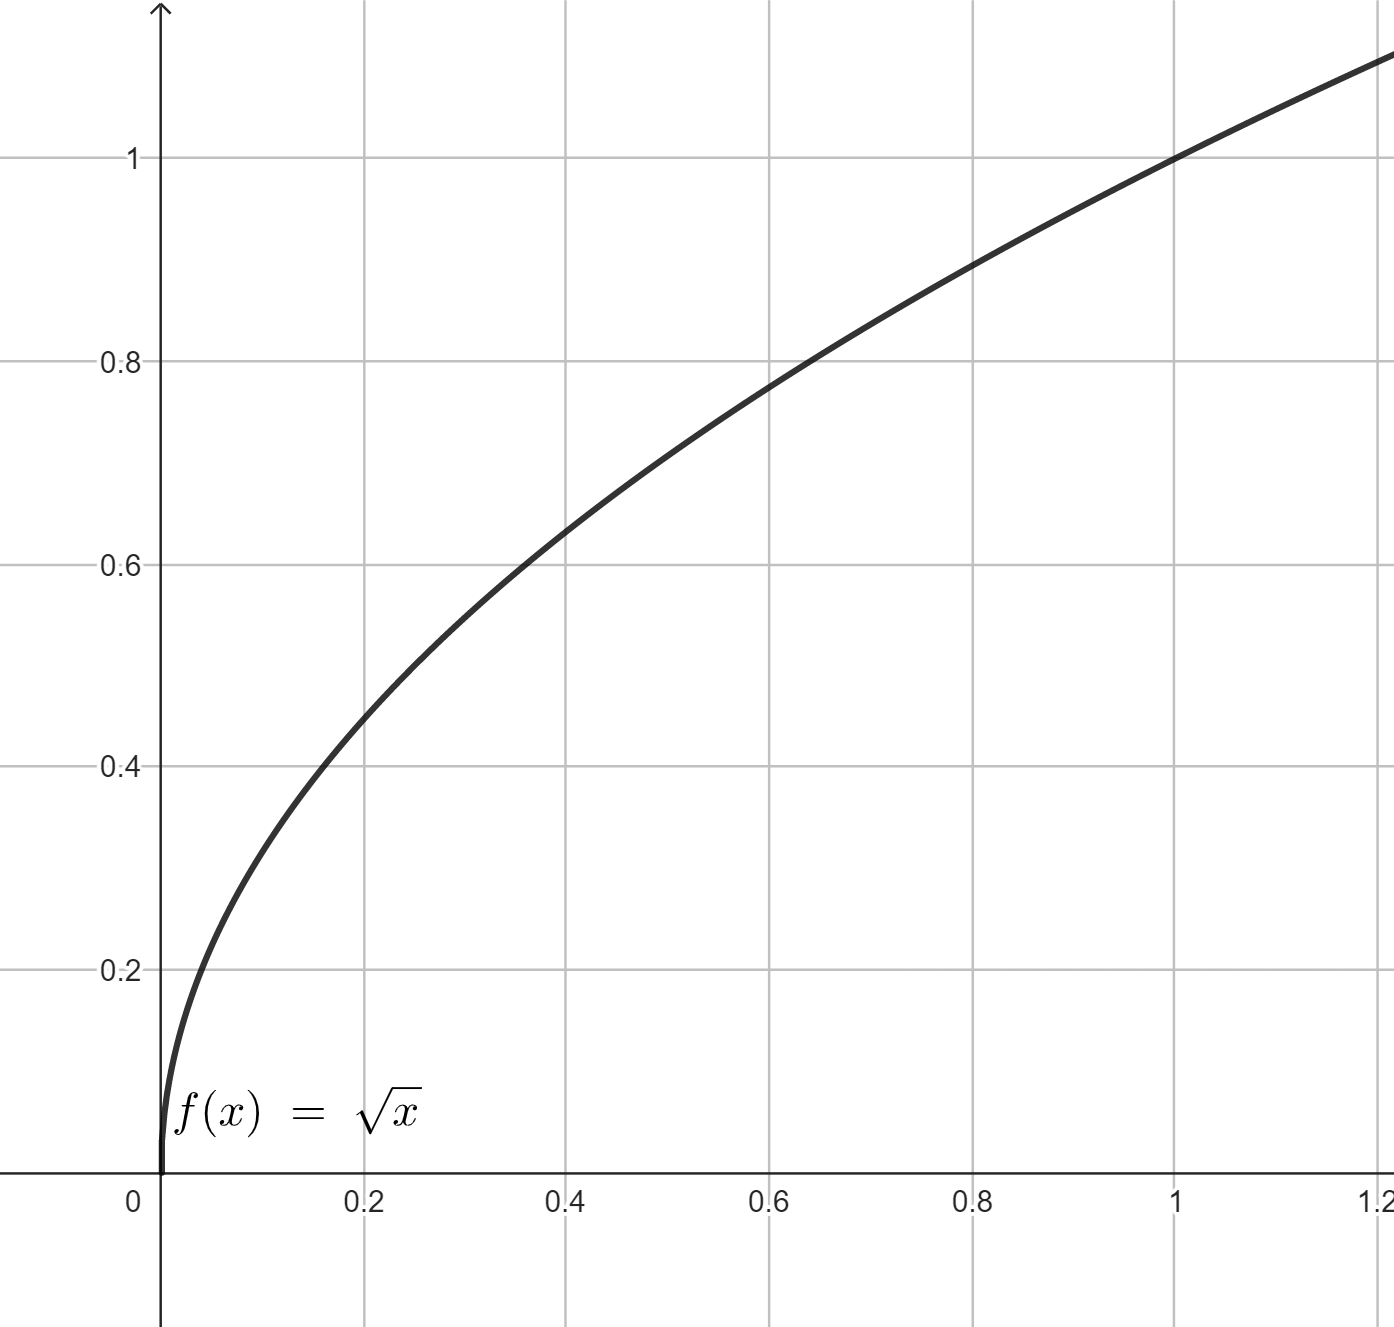
\includegraphics[width=0.75\linewidth]{Images/sqrtx.png}
    \caption{$f(x)=\sqrt{x}$}
\end{wrapfigure}

A expresión da derivada k-ésima non se pode avaliar se $k>m$ e a derivada nunca se anula (Só se anula se $m\in\mathbb{N}$), xa que temos unha indeterminación do tipo $[\frac{k}{0}]$. A idea intuitiva disto é que a recta tanxente ten pendente infinita cando $x\to 0$. Podemos velo gráficamente coa función $f(x)=\sqrt{x}$. En $x_0=0$ a pendente da recta tanxente vaise ao infinito, polo que non é derivable, aínda que si que exista $f(0)$.

\par Podemos aplicar esta lóxica e buscar solucións non analíticas en $x_0$ para ecuacións de segunda orde máis xerais, do tipo de:

\begin{equation*}
    y^{\prime \prime}+\frac{p_{0}+p_{1} x+p_{2} x^{2}+\cdots}{x} y^{\prime}+\frac{q_{0}+q_{1} x+q_{2} x^{2}+\cdots}{x^{2}} y=0
\end{equation*}

En este tipo de ecuacións, cando $x<<<1$ os termos $p_0$ e $q_0$ dominarán nos numeradores, facendo que podamos despreciar aos outros termos con potencias de $n$ e buscar solucións do tipo $x^m$, como se tratáramos cunha ecuación de Euler. En certos casos que estudaremos a continuación as ED deste tipo poden resolverse por series de potencias, obtendo solucións do tipo:

\begin{equation*}
    y=x^{m}\left(a_{0}+a_{1} x+a_{2} x^{2}+\cdots\right)=x^{m} \sum_{n=0}^{\infty} a_{n} x^{n} \quad m \in \mathbb{R}
\end{equation*}

Este tipo de series de potencias denomínanse \textbf{series de Frobenius}.

\subsection{Clasificación e estudo dos puntos non regulares}

Sexa $x=x_{0}$ un punto singular da ecuación diferencial:

$$
y^{\prime \prime}+P(x) y^{\prime}+Q(x) y=0
$$

\begin{mydef}
    Dise que $x_{0}$ é un punto singular regular da ecuación diferencial se as funcións $(x-$ $\left.x_{0}\right) P(x)$ e $\left(x-x_{0}\right)^{2} Q(x)$ son analíticas en $x=x_{0}$. Se algunha destas funcións non é analítica, dise que $x_{0}$ é un punto singular irregular.
\end{mydef}

Supoñendo que $x_0=0$ é un punto singular regular na nosa ecuación de partida vamos a tratar de resolver a ED por series de Frobenius. Trataremos de determinar cando obteremos dúas solucións LI e cando existirá solo unha (Th. de Fuchs):

$$
\begin{aligned}
y & =x^{m} \sum_{n=0}^{\infty} a_{n} x^{n}=\sum_{n=0}^{\infty} a_{n} x^{m+n} \Rightarrow \\
y^{\prime} & =\sum_{n=0}^{\infty}(m+n) a_{n} x^{m+n-1} \Rightarrow \\
y^{\prime \prime} & =\sum_{n=0}^{\infty}(m+n)(m+n-1) a_{n} x^{m+n-2}=x^{m-2} \sum_{n=0}^{\infty}(m+n)(m+n-1) a_{n} x^{n}
\end{aligned}
$$

O seguinte paso é tratar de expresar as funcións $P(x)$ e $Q(x)$ como unha serie de Taylor para substituír todas as series na ecuación e poder operar con elas. Unha vez convertidas as funcións en series de Taylor temos que operar o producto entre a serie de Taylor e a expresión en forma de serie da derivada n-ésima da función.  O exemplo do produto de $Q(x)$ e $y$ será representado a continuación, en forma de táboa:

$$
\begin{aligned}
    Q(x) y & =\frac{1}{x^{2}}\left[\sum_{n=0}^{\infty} q_{n} x^{n}\right]\left[\sum_{n=0}^{\infty} a_{n} x^{n}\right] x^{m} \\
    & =x^{m-2} \sum_{n=0}^{\infty}\left[\sum_{k=0}^{n} q_{n-k} a_{k}\right] x^{n}
\end{aligned}
$$

Para operar buscamos agrupar as diagonais coa mesma potencia de $x$:

$$
\begin{array}{c|l} 
& a_{0}+a_{1} x+a_{2} x^{2}+a_{3} x^{3}+\cdots=\sum_{n=0}^{\infty} a_{n} x^{n} \\
\hline q_{0} & q_{0} a_{0}+q_{0} a_{1} x+q_{0} a_{2} x^{2}+q_{0} a_{3} x^{3}+\cdots \\
+q_{1} x & +q_{1} a_{0} x+q_{1} a_{1} x^{2}+q_{1} a_{2} x^{3}+ \\
+q_{2} x^{2} & +q_{2} a_{0} x^{2}+q_{2} a_{1} x^{3}+ \\
+q_{3} x^{3} & +q_{3} a_{0} x^{3}+ \\
\vdots & \vdots \\
=\sum_{n=0}^{\infty}q_nx^n &
\end{array}
$$

$$
\begin{aligned}
P(x) y^{\prime} & =\frac{1}{x}\left[\sum_{n=0}^{\infty} p_{n} x^{n}\right]\left[\sum_{n=0}^{\infty}(m+n) a_{n} x^{m+n-1}\right] \\
& =x^{m-2}\left[\sum_{n=0}^{\infty} p_{n} x^{n}\right]\left[\sum_{n=0}^{\infty}(m+n) a_{n} x^{n}\right] \\
& =x^{m-2} \sum_{n=0}^{\infty}\left[\sum_{k=0}^{n} p_{n-k}(m+k) a_{k}\right] x^{n}
\end{aligned}
$$

Agora facemos a substitución que anunciábamos, sacamos factor común $x^{m-2}$ e unimos os sumatorios con índice $n$ :

$$
x^{m-2} \sum_{n=0}^{\infty}\left\{(m+n)(m+n-1) a_{n} x^{n}+\left[\sum_{k=0}^{n} p_{n-k}(m+k) a_{k}\right] x^{n}+\left[\sum_{k=0}^{n} q_{n-k} a_{k}\right] x^{n}\right\}=0
$$

Dentro do sumatorio sacamos factor común $x^{n}$ e agrupamos os sumatorios interiores:

$$
\sum_{n=0}^{\infty}\left\{(m+n)(m+n-1) a_{n}+\sum_{k=0}^{n}\left[p_{n-k}(m+k)+q_{n-k}\right] a_{k}\right\} x^{n}=0
$$

Nesta expresión temos a serie de Taylor igualada á función 0, polo que podemos afirmar que todos os termos da serie valen 0:

\begin{equation*}
    (m+n)(m+n-1) a_{n}+\sum_{k=0}^{n}\left[p_{n-k}(m+k)+q_{n-k}\right] a_{k} = 0
\end{equation*}

Esta expresión depende do valor de $n$ no que nos atopemos, estudaremos en primeiro lugar o caso máis simple, $n=0$ (Supoñendo sen perda de xeralidade que $a_0 \neq 0$):

\begin{equation*}
    m(m-1)+m p_{0}+q_{0}=0\Rightarrow m^{2}+m\left(p_{0}-1\right)+q_{0}=0
\end{equation*}

Esta ecuación denomínase ecuación indicial e nos permitirá calcular os valores de $m$ válidos. Garda unha relación moi estreita coa ecuación característica das ED de Euler, que obtemos despois de facer a substitución $y=x^m$ para buscar solucións en forma de potencias.

\par Se en vez de $n=0$ estudamos o resto dos casos obteremos ecuacións que nos relacionan, en xeral, cada término $a_n$ cos $n$ términos anteriores $(a_0,a_{n-1})$. Por exemplo para $n=1$ obtemos:

\begin{equation*}
    \begin{gathered}
        (m+1) m a_{1}+\left[p_{1} m+q_{1}\right] a_{0}+\left[p_{0}(m+1)+q_{0}\right] a_{1}=0, \Rightarrow \\
        {\left[(m+1)\left(m+p_{0}\right)+q_{0}\right] a_{1}=-\left[p_{1} m+q_{1}\right] a_{0}}
    \end{gathered}
\end{equation*}

Esta ecuación relaciona $a_1$ con $a_0$, podemos despexar $a_1$ se $(m+1)(m+p_0)q_0 \neq 0$. Podemos obter a ecuación xeral de recorrencia para todos os valores de $n$ se calculamos o termo que acompaña a $a_n$ e o sacamos do sumatorio:

\begin{equation*}
    \sum_{k=0}^{n}\left[p_{n-k}(m+k)+q_{n-k}\right] a_{k} = [(m+n)p_0+q_0]a_n + \sum_{k=0}^{n-1}\left[p_{n-k}(m+k)+q_{n-k}\right] a_{k}
\end{equation*}

Polo tanto obtemos a seguinte ecuación de recorrencia para $n\geq 0$:

\begin{equation*}
    \left[(m+n)(m+n-1)+(m+n) p_{0}+q_{0}\right] a_{n}+\sum_{k=0}^{n-1}\left[p_{n-k}(m+k)+q_{n-k}\right] a_{k}=0 \quad n=1,2, \ldots
\end{equation*}

Para poder obter $a_n$ en función do termo anterior o coeficiente que o acompaña debe ser distinto de 0. Para estudar cando isto ocorre ou non vamos a definir a seguinte función:

\begin{equation*}
    f(m)=m(m-1)+m p_{0}+q_{0}
\end{equation*}

Se representamos esta función obtemos unha parábola cuxos ceros están situados nos valores $m_1$ e $m_2$, onde $m_1\geq m_2$. Esta función está definida para que o seu valor coincida co coeficiente que acompaña a cada termo $a_i$ cando calculamos $f(m+i)$. Por exemplo, queda claro cando calculamos o valor de $f(m+n)$:

\begin{equation*}
    f(m+n) = \left[(m+n)(m+n-1)+(m+n) p_{0}+q_{0}\right]
\end{equation*}

A partir desta función podemos escribir a relación de recorrencia para os 5 primeiros valores de $n$:

$$
\begin{aligned}
& f(m+1) a_{1}+\left(p_{1} m+q_{1}\right) a_{0}=0 \\
& f(m+2) a_{2}+\left(p_{2} m+q_{2}\right) a_{0}+\left[p_{1}(m+1)+q_{1}\right] a_{1}=0 \\
& f(m+3) a_{3}+\left(p_{3} m+q_{3}\right) a_{0}+\left[p_{2}(m+1)+q_{2}\right] a_{1}+\left[p_{1}(m+2)+q_{1}\right] a_{2}=0
\end{aligned}
$$

Polo tanto podemos concluir que o coeficiente de $a_n$ é $f(m+n)$. Ese valor de $m$ só pode ser $m_1$ ou $m_2$, as solucións da ecuación indicial. Se tomamos o maior dos valores de $m$, $m_1$, entón $f(m_1+n)$ nunca se anula porque $n>0$. Se tomamos $m_2$ podemos enfrentarnos a tres posibles situacións:

\begin{itemize}
    \item Se $m_{1}=m_{2}$ a segunda solución non se pode expresar como serie de Frobenius.
    \item Se $m_{1}-m_{2}=L \in \mathbb{N}^{+}, f\left(m_{2}+L\right)=f\left(m_{2}+m_{1}-m_{2}\right)=0$, entón $a_{L}$ desaparece da ecuación $L$-ésima, quedándonos $L$ ecuacións lineais homoxéneas con $L$ incógnitas. Agora ben: 
    \begin{itemize}
        \item Se son linealmente dependentes, podemos prescindir da ecuación para $n=$ $L$, polo que $a_{L}$ quedaría libre, podendo tomar calquera valor (por exemplo cero). Coas ecuacións para $n=L+1$ e sucesivas, calcularíamos os valores de $a_{L+1}, a_{L+2} \ldots$
        \item Se estas ecuacións son linealmente independentes, a única solución posible é $a_{0}=a_{1}=\ldots=a_{L-1}=0$ en contradición coa hipótese. Poderíamos pensar que agora tamén somos libres para asignar calquera valor a $a_{L}$ e proseguir coas seguintes ecuacións, pero estariamos construíndo outra vez a solución para $m_{1}$.
    \end{itemize}
    \item Se $m_{1}-m_{2}=L \notin \mathbb{N}$, tamén podemos calcular os coeficientes para $m_{2}$, o menor dos dous valores de $m$.
\end{itemize}

\subsection{Teorema de Fuchs}

\begin{theorem}
    Supoñamos que $x=x_{0}$ é un punto singular regular da ecuación diferencial (2): $y^{\prime \prime}+$ $P(x) y^{\prime}+Q(x)=0$, e que os desenvolvementos en serie de potencias de $\left(x-x_{0}\right) P(x)$ e $\left(x-x_{0}\right)^{2} Q(x)$ converxen para $\left|x-x_{0}\right|<R$ con $R>0$. Sexan $m_{1}$ e $m_{2}$ as raíces da ecuación indicial (4) con $m_{2} \leq m_{1}$. Entón a ecuación diferencial ten polo menos unha solución en serie de Frobenius:

$$
y_{1}=\sum_{n=0}^{\infty} a_{n}\left(x-x_{0}\right)^{m_{1}+n}
$$

válida en $\left|x-x_{0}\right|<R$, onde os $a_{n}$ quedan determinados en función de $a_{0} \neq 0$ pola fórmula de recorrencia (5). Ademais, se $m_{1}-m_{2}$ non é un enteiro positivo ou cero, a ecuación diferencial ten unha segunda solución independente:

$$
y_{2}=\sum_{n=0}^{\infty} b_{n}\left(x-x_{0}\right)^{m_{2}+n}
$$

válida no mesmo intervalo, onde de novo $b_{0} \neq 0$ e $b_{n}$ ven dado unha fórmula de recorrencia análoga.
\end{theorem}

\section{Ecuación de Bessel}

Consideremos a familia de ecuacións diferenciais:

$$
x^{2} y^{\prime \prime}+x y^{\prime}+\left(x^{2}-p^{2}\right) y=0 \quad p \geq 0, p \in \mathbb{R} .
$$

Escrita en forma normal:

$$
y^{\prime \prime} + \frac{1}{x} y^{\prime} + \left (1-\frac{p^2}{x^2}\right ) y = 0
$$

En primeiro lugar vamos a estudar o comportamento xeral da ecuación, para poder facernos unha idea de cales poden ser as súas solucións en función da relación entre $x$ e $p$:

\begin{itemize}
    \item Se $x<<<p$ o termo $x^2$ perde importancia frente a $p^2$, polo que a ED acaba parecendo unha ED de Euler, que admite solucións do tipo $y=x^m$.
    \item Se $x>>>p$ podemos desprezar o termo $\frac{1}{x}y$ e aproximar a ED a outra máis coñecida: $y^{\prime \prime} + y =0$. Esta ecuación admite solucións do tipo $y=A\cos x + B\sin x$, funcións periódicas.
\end{itemize}

Na seguinte figura podemos ver representadas varias solucións da ecuación de Bessel:

\begin{figure}[h!]
    \centering
    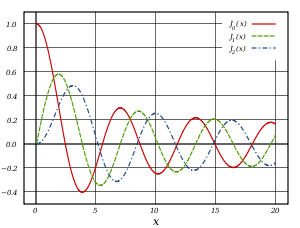
\includegraphics[width=0.75\linewidth]{Images/bessel.png}
    \caption{Funcións de Bessel para $p=0,1,2$}
\end{figure}

O punto $x_0=0$ non é ordinario, pero si que é singular regular xa que cumple que:

$$
x P(x)=1 \quad \text { e } \quad x^{2} Q(x)=x^{2}-p^{2}
$$

son funcións analíticas con radio de converxencia infinito. Entón ten que existir polo menos unha solución en forma de serie de Frobenius (Th. de Fuchs). Para buscar esta solución vamos a calcular a forma que teñen todos os termos que participan na ED a partir da expresión base da serie de Frobenius:

\begin{equation*}
    \begin{gathered}
        y = x^{m}\sum_{n=0}^{\infty}a_{n} x^{n}=\sum_{n=0}^{\infty} a_{n} x^{n+m}  \Rightarrow  x^{2} y=\sum_{n=0}^{\infty} a_{n} x^{n+m+2}=\sum_{n=2}^{\infty} a_{n-2} x^{n+m}\\
        y^{\prime} =  \sum_{n=0}^{\infty}(n+m) a_{n} x^{n+m-1}  \Rightarrow  x y^{\prime}=\sum_{n=0}^{\infty}(n+m)a_{n} x^{n+m} \\
        y^{\prime \prime} = \sum_{n=0}^{\infty}(n+m)(n+m-1) a_{n} x^{n+m-2}  \Rightarrow  x^2y^{\prime \prime} = \sum_{n=0}^{\infty}(n+m)(n+m-1) a_{n} x^{n+m}
    \end{gathered}
\end{equation*}

No cálculo de $x^2y$ fixemos un cambio de índice $n^{\prime}=n-2$, que nos servirá para agrupar potencias de $x$ cando substituámos as series na ED. Podemos facer este cambio de índice porque é unha variable muda, que só pertence ao sumatorio. Unha idea intuitiva para velo é que adiantamos o índice dúas unidades e rebaixamos o interior do sumatorio en dúas unidades. Se substituímos todas as series na ecuación de Bessel obtemos:

$$
\underbrace{\sum_{n=0}^{\infty}(n+m)(n+m-1) a_{n} x^{n+m}}_{x^{2} y^{\prime \prime}}+\underbrace{\sum_{n=0}^{\infty}(n+m) a_{n} x^{n+m}}_{x y^{\prime}}+\underbrace{\sum_{n=2}^{\infty} a_{n-2} x^{n+m}}_{x^{2} y}-\underbrace{\sum_{n=0}^{\infty} p^{2} a_{n} x^{n+m}}_{p^{2} y}=0
$$

Podemos agrupar o primeiro, segundo e cuarto sumatorio xa que empezan en $n=0$. Sacando factor común $x^m$ en todos os sumatorios obtemos:

$$
x^{m}\left\{\sum_{n=0}^{\infty}\left[(n+m)^{2}-p^{2}\right] a_{n} x^{n}+\sum_{n=2}^{\infty} a_{n-2} x^{n}\right\}=0 .
$$

O seguinte paso é agrupar todos os sumatorios, pero precisamos sacar os dous primeiros termos do primeiro sumatorio para que teñan o mesmo índice inicial:

$$
\begin{aligned}
& {\left[m^{2}-p^{2}\right] a_{0}+\left[(m+1)^{2}-p^{2}\right] a_{1} x+\sum_{n=2}^{\infty}\left[(n+m)^{2}-p^{2}\right] a_{n} x^{n}+\sum_{n=2}^{\infty} a_{n-2} x^{n}=0 \Rightarrow} \\
& {\left[m^{2}-p^{2}\right] a_{0}+\left[(m+1)^{2}-p^{2}\right] a_{1} x+\sum_{n=2}^{\infty}\left\{\left[(n+m)^{2}-p^{2}\right] a_{n}+a_{n-2}\right\} x^{n}=0 .}
\end{aligned}
$$

\end{document}